% Copyright 2005-2016 Airbus-EDF-IMACS-Phimeca
% Permission is granted to copy, distribute and/or modify this document
% under the terms of the GNU Free Documentation License, Version 1.2
% or any later version published by the Free Software Foundation;
% with no Invariant Sections, no Front-Cover Texts, and no Back-Cover
% Texts.  A copy of the license is included in the section entitled "GNU
% Free Documentation License".
\renewcommand{\filename}{docUC_TimeSeries.tex}
\renewcommand{\filetitle}{UC : Manipulation of a time series}

% \HeaderNNIILevel
\HeaderIILevel
%\HeaderIIILevel

\label{UCtimeSeries}

\index{Stochastic Process!Time Series}


The objective here is to create and manipulate a time series. A time series is a particular field where the mesh $\cM$ can be considered as a regular time grid  $(t_0, \dots, t_{N-1})$.\\

The spatial mean of a time series corresponds to a temporal mean and is evaluated as  defined in (\ref{spatMeanField}). \\

It is possible to draw a time series, using interpolation between the values: see the use case on the Field.\\

A  time series can be obtained as a realization of a multivariate stochastic process  $X: \Omega \times [0,T] \rightarrow \Rset^d$   of dimension $d$ where $[0,T]$ is discretized according to the regular grid $(t_0, \dots, t_{N-1})$ . The  values $(\vect{x}_0, \dots, \vect{x}_{N-1})$ of the  time series are defined by:
\begin{align}
  \forall i \in [0, N-1],\quad   \vect{x}_i= X(\omega)(t_i)
\end{align}

A time series is stored in the \emph{TimeSeries} object that stores the regular time grid and the associated values.\\



\requirements{
  \begin{description}
  \item[$\bullet$] a time grid : {\itshape \textit{myTimeGrid}}
  \item[type:]  RegularGrid
  \end{description}


  \begin{description}
  \item[$\bullet$] some values  : {\itshape \textit{myValues}}
  \item[type:]  NumericalSample
  \end{description}

}
{
  \begin{description}
  \item[$\bullet$] a time series : {\itshape myTimeSeries}
  \item[type:]  TimeSeries
  \end{description}
}

\textspace\\
Python script for this UseCase :

\inputscript{script_docUC_StocProc_TimeSeries}

\textspace\\
Consider the temporal normal process of dimension~1 which covariance model is $Exponential(a,\lambda)$ with $(a, \lambda)=(1.0, 0.2)$ and the  time grid $[0,1]$ regularly discretized with 101 points. \\
We draw  a realization of this process on the time grid using no interpolation: see  Figure \ref{TS1} and using a linear interpolation: see  Figure \ref{TS2}.


\begin{figure}[H]
  \begin{minipage}{9cm}
    \begin{center}
      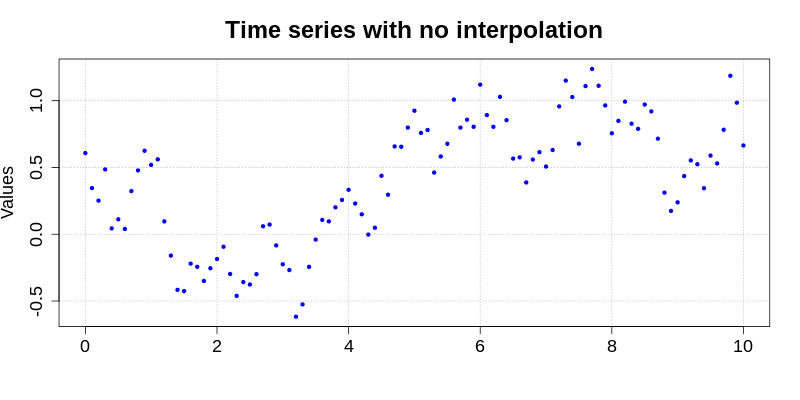
\includegraphics[width=6cm]{Figures/timeSeriesNoInterp.png}
      \caption{One time series with no interpolation.}
      \label{TS1}
    \end{center}
  \end{minipage}
  \hfill
  \begin{minipage}{9cm}
    \begin{center}
      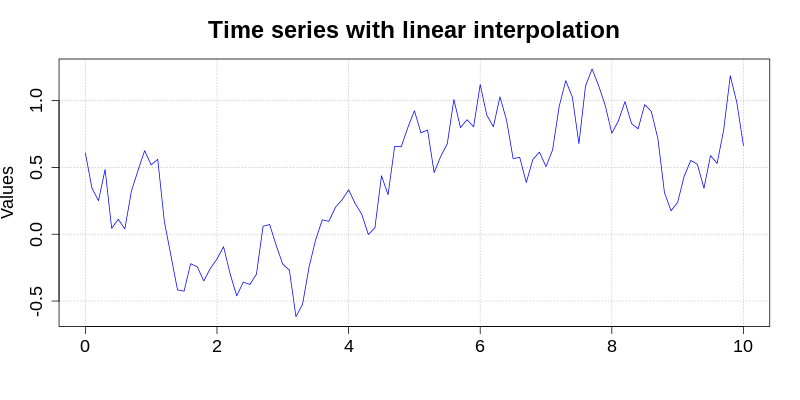
\includegraphics[width=6cm]{Figures/timeSeriesInterp.png}
      \caption{Time series of Figure \ref{TS1} using linear interpolation.}
      \label{TS2}
    \end{center}
  \end{minipage}
\end{figure}
